\documentclass[a4paper]{article}
\usepackage{titling}
\usepackage{authblk}
\usepackage{fancyhdr}
\usepackage{hyperref}
\usepackage{rsc}
\usepackage{siunitx}
\usepackage{graphicx}
\usepackage{listings}
\usepackage{amsmath}
\usepackage{color}

\definecolor{dkgreen}{rgb}{0,0.6,0}
\definecolor{gray}{rgb}{0.5,0.5,0.5}
\definecolor{mauve}{rgb}{0.58,0,0.82}


\lstset{frame=tb,
  language=Python,
  aboveskip=3mm,
  belowskip=3mm,
  showstringspaces=false,
  columns=flexible,
  basicstyle={\ttfamily},
  numbers=none,
  numberstyle=\tiny\color{gray},
  keywordstyle=\color{blue},
  commentstyle=\color{dkgreen},
  stringstyle=\color{mauve},
  breaklines=true,
  breakatwhitespace=true,
  tabsize=3
}
\DeclareSIUnit\Fahrenheit{\degree F}
\setlength{\parindent}{0pt}
\parskip 1.5ex

\title{Problem Solving Handout 1: Protein helix to coil transition}
\author[1]{Dr Benjamin J. Morgan}
\author[1,2]{Dr Andrew R. McCluskey}
\affil[1]{Department of Chemistry, University of Bath, email: b.j.morgan@bath.ac.uk}
\affil[2]{Diamond Light Source, email: andrew.mccluskey@diamond.ac.uk}
\setcounter{Maxaffil}{0}
\renewcommand\Affilfont{\itshape\small}

\pagestyle{fancy}
\fancyhf{}
\rhead{CH40208}
\lhead{\thetitle}
\rfoot{\thepage}

\begin{document}
\maketitle

The focus of this exercise is to give you experience of applying programming to an abstract chemical problem. 
This exercise will involve a substantial amount of problem solving, and will be similar in style to the examination at the end of the module. 
This handout provides necessary background to help you solve the problem that is detailed in the Problem Solving Exercise 1 sheet. \\
\linebreak
\textbf{Read through this material completely before the session on X-DATE-GOES-HERE-X}.

\section{Background}

Proteins are polymers molecules of biochemical importance, the specific biochemistry of a particular protein is heavily influenced by their three dimensional structure. 
The particular monomers which make up protein molecules are known as amino acids. 
These individual amino acids are able to form secondary structures through complex hydrogen bonding networks, these are secondary to the covalently bonded amino acids. 
The most common secondary structures are $\alpha$-helices and $\beta$-sheets, examples of these are shown in Figure~\ref{fig:ss}. 
Under certain conditions, these secondary structures can undergo collapse into a random coil. 
The unwinding of an $\alpha$-helix into a random coil is a \texttt{cooperative transition}, in which the helix becomes increasingly suspectible to structure changes once the process has begun. 
Statistical thermodynamics can be used to develop a model that describes the probability of this transition while accounting for the cooperativiely of the occurance. 

\begin{figure}
  \centering
  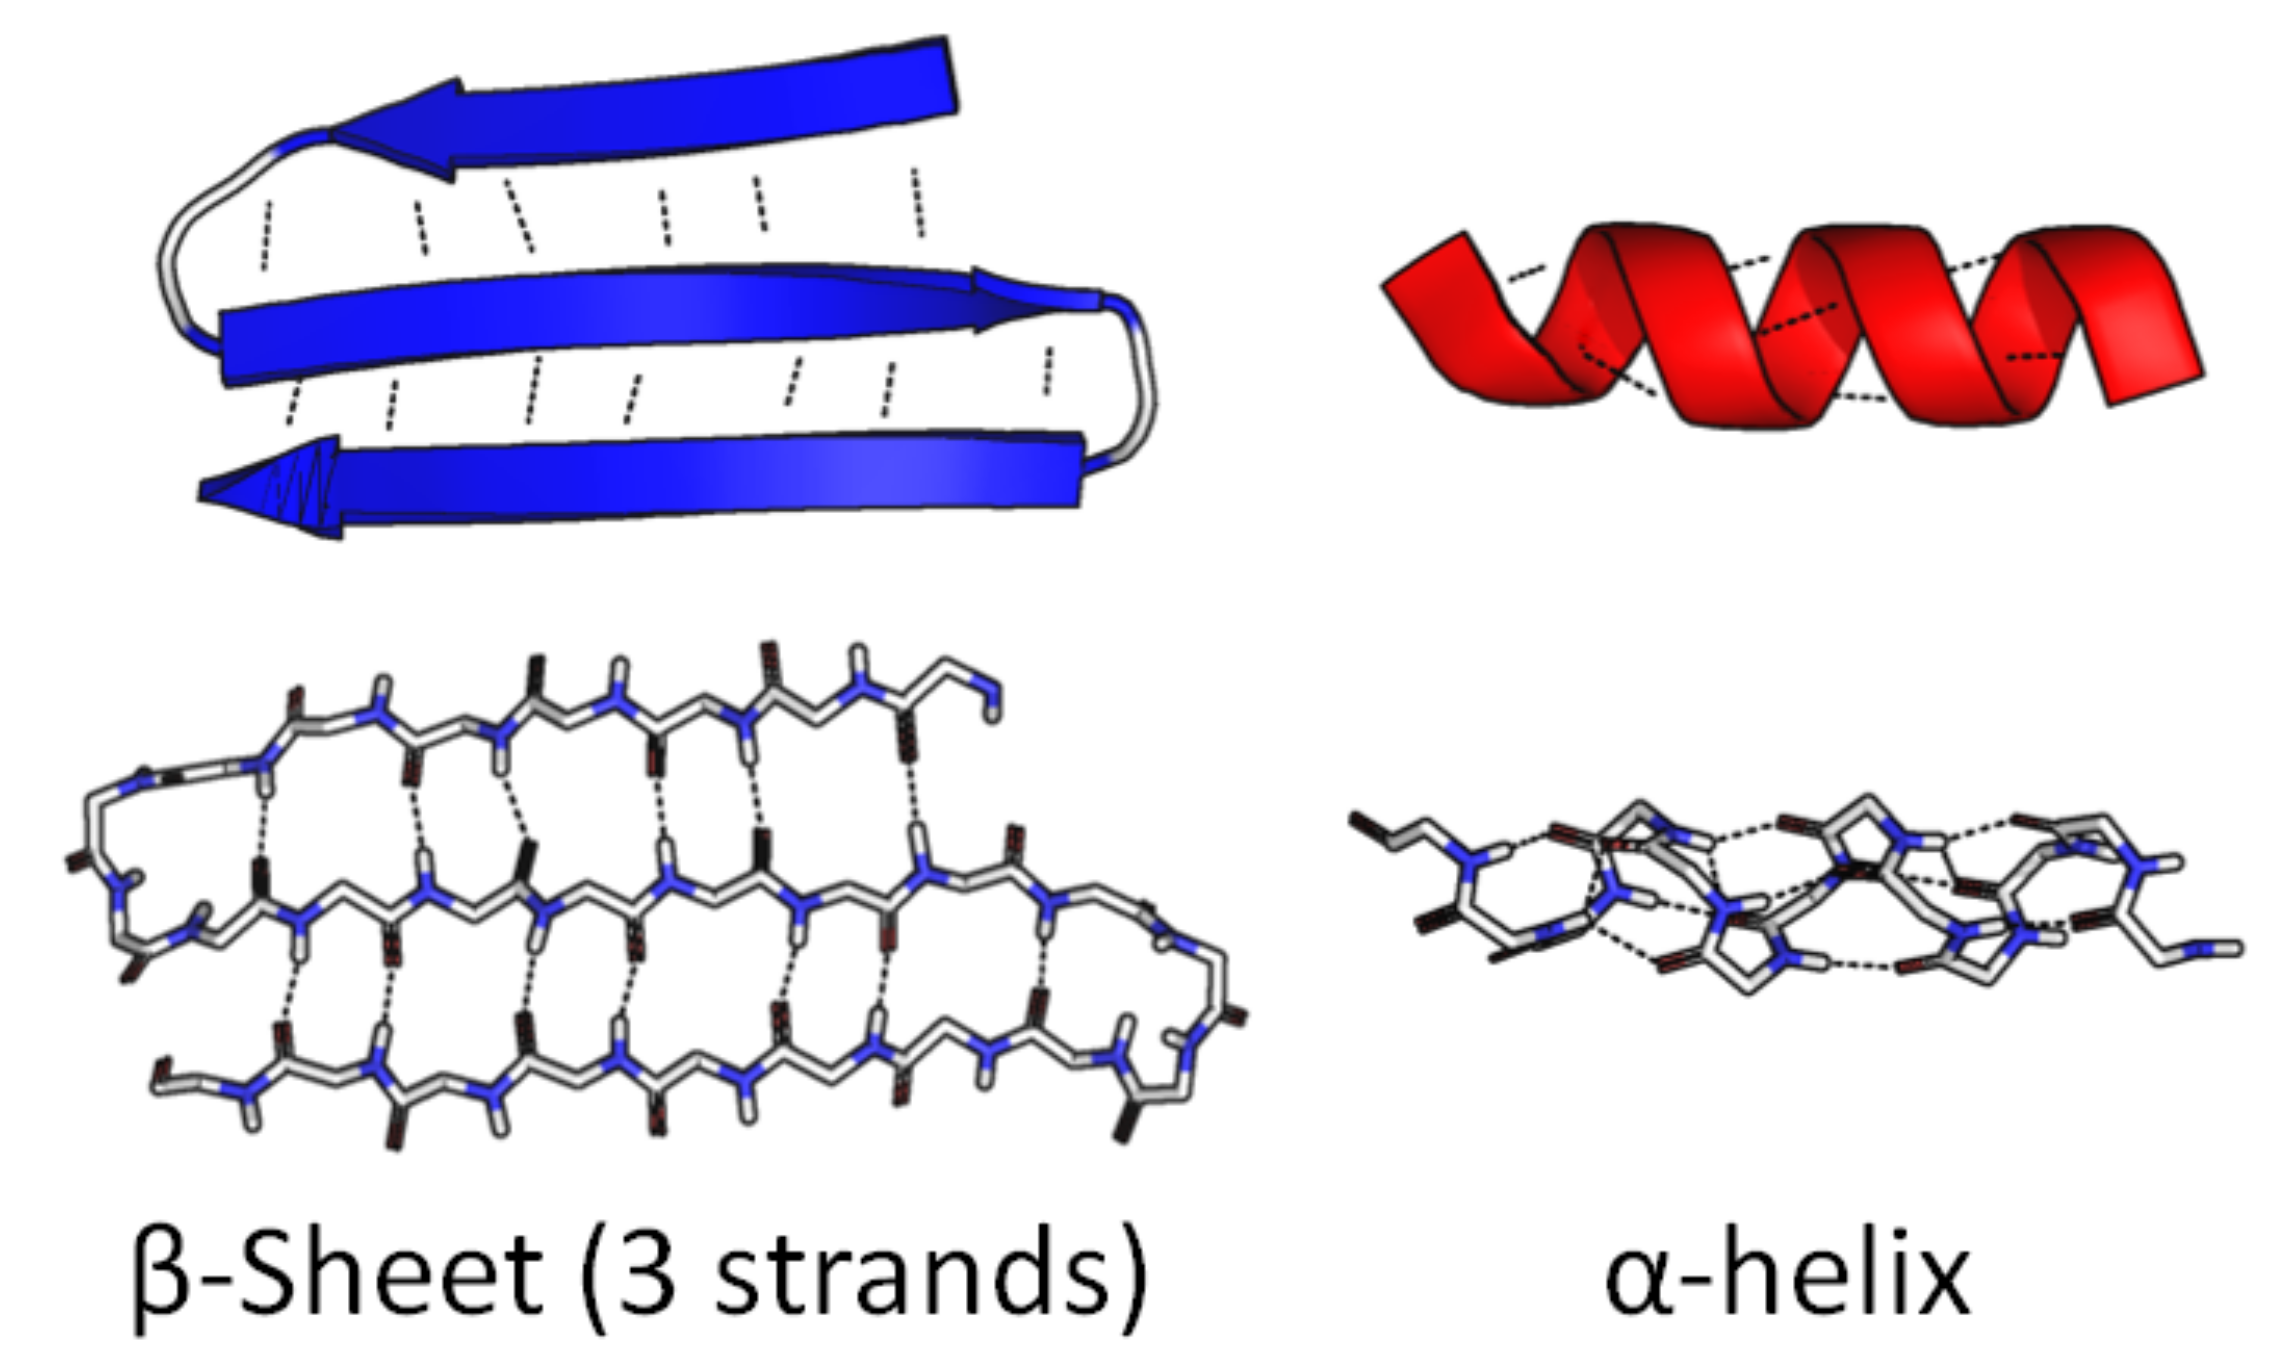
\includegraphics[width=0.8\textwidth]{secondary_structure}
  \caption{\label{fig:ss} Examples of the secondary structures formed by amino acids, the hydrogen bonding is represented by dashed black lines. Figure by Thomas Shafee, distributed under a CC BY-SA 4.0 license.}
\end{figure}
%

\section{Small protein}
In order to evaluate the fraction of amino acids present in a random coil or an $\alpha$-helix it is necessary to set up the paritition function for the various states of the molecule. 
Considering first a short protein consisting of four amino acids, each of which can either be in a coil, $c$, or a helix, $h$. 
When the configuration is $hhhh$, the partition coefficient will be termed, $q_0$, while if the configuration is $cccc$ the partition coefficient will be termed $q_4$. 
The total partition function ($q$) is therefore, 
%
\begin{equation}
    q = C(4, 0) q_0 + C(4, 1) q_1 + C(4, 2) q_2 + C(4, 3) q_3 + C(4, 4) q_4,
    \label{equ:part}
\end{equation}
%
where, $C(n, i)$ gives the number of permutations of $i$ random coil amino acids in $n$ total amino acids. 
This can be found with the following relationship,
%
\begin{equation}
    C(n, i) = \frac{n!}{(n-i)!i!}, 
\end{equation}
%
where, $!$ indicates that the \emph{factorial} is being taken. 
Equation \ref{equ:part} may be rewritten as,
%
\begin{equation}
    q = q_0\bigg(C(4, 0) + \frac{C(4, 1) q_1}{q_0} + \frac{C(4, 2) q_2}{q_0} + \frac{C(4, 3) q_3}{q_0} + \frac{C(4, 4) q_4}{q_0}\bigg),
    \label{equ:part1}
\end{equation}
%
from which, we can suppose that each partition function differs from $q_0$ only by the energy of each conformation relative to $hhhh$, therefore, 
%
\begin{equation}
    \frac{q_i}{q_0} = \exp{\bigg(\frac{-(\varepsilon_i - \varepsilon_0)}{kT}\bigg)},
    \label{equ:part2}
\end{equation}
%
where, $\varepsilon_i - \varepsilon_0$ is the transition energy from $0$ to $i$, $k$ is the Boltzmann constant, and $T$ is the temperature.

\section{Non-cooperative model}
In order to generalise this for any number of amino acids, we will first consider the case where the $\alpha$-helix to random coil transitions are non-cooperative. 
This means that the energy associated with changing one $h$ amino acid to a $c$ amino acid is the same, regardless of how many $h$ or $c$ amino acids are already present. 
The energy change between $c^ih^{4-i}$ and $c^{i+1}h^{3-i}$ is the same, $\gamma$ for any value of $i$, which implies that $\varepsilon_i - \varepsilon_0 = i\gamma$.
By bringing together Equations~\ref{equ:part1},~\ref{equ:part2}, and the above assumption, we can write the total partition function as,
%
\begin{equation}
    \begin{aligned}
        q = q_0\Bigg[&C(4, 0) + C(4, 1) \exp{\bigg(\frac{-\gamma}{kT}\bigg)} + C(4, 2) \exp{\bigg(\frac{-2\gamma}{kT}\bigg)} \\
         & + C(4, 3) \exp{\bigg(\frac{-3\gamma}{kT}\bigg)} + C(4, 4) \exp{\bigg(\frac{-4\gamma}{kT}\bigg)}\Bigg], \\
        q = q_0(&C(4, 0) + C(4, 1) s + C(4, 2) s^2 + C(4, 3) s^3 + C(4, 4) s^4), \\
    \end{aligned}
    \label{equ:parent}
\end{equation}
%
where, 
%
\begin{equation}
    s = \exp{\bigg(\frac{-\gamma}{kT}\bigg)},
\end{equation}
%
which is known as the stability parameter. 
The term within the parenthesis on the last line of Equation~\ref{equ:parent} has the form of the binomial expansion of $(1 + s)^4$. 

The binomial expansion of $(1 + x)^n$ is, 
%
\begin{equation}
    (1 + x)^n = \sum_{i=0}^{n}C(n, i)x^i.
\end{equation}
%
Therefore it is possible to rewrite Equation~\ref{equ:parent} as, 
%
\begin{equation}
    \frac{q}{q_0} = \sum_{i=0}^{4}C(4, i)s^i.
\end{equation}
%
This can be generalised to a protein molecule of any number of amino acids, 
%
\begin{equation}
    \frac{q}{q_0} = \sum_{i=0}^{n}C(n, i)s^i.
\end{equation}
%

\section{Cooperative model}

The application of a cooperative model is more complex, as it depends on modelling how neighbours facilities each other's comnformational change. 
The \emph{zipper} model only allows for the conversion of $h$ to $c$ is an amino acid adjacent has already undergone the change. 
So the following, 
%
\begin{equation*}
    \ldots hhhch \ldots \rightarrow \ldots hhcch \ldots, 
\end{equation*}
%
is an allowed transition. 
However, 
%
\begin{equation*}
    \ldots hhhch \ldots \rightarrow \ldots hchch \ldots, 
\end{equation*}
%
is not.
Of course, for this to be possible, the first conversion must not have this rule applied (or else the collapse would be impossible). 
Cooperativity is included in the zipper model by the assuming that the \emph{nucleation step}, the first transition, is less favourable than the remaining conversions. 
Therefore, for the nucleation step, the stability parameter is multiplied by some parameter $\sigma$, where $\sigma \ll 1$.
Each subquent, \emph{propagation} step has a stability parameter of $s$. 
This leads to a functional description of the partition function, 
%
\begin{equation}
    q = 1 + \sigma(n + 1)\sum_{i=1}^{n}s^i - \sigma\sum_{i=1}{n}s^i
\end{equation}
%
The fraction, $p_i$, of molecules that has $i$ amino acids in the coil conformation can be found as, 
%
\begin{equation}
    p_i = \frac{(n - i + 1) \sigma s^i}{q},
\end{equation}
and the mean value of $i$ is found as $\langle i \rangle = \sum_i ip_i$. 

\bibliographystyle{rsc}
\bibliography{handout_2}

\end{document}
